% ==========================================
% BASE KNOWLEDGES
% ==========================================

\newpage
\chapter{KIẾN THỨC NỀN}

\begin{concept}[15cm]
\textit{Nội dung chương này sẽ giới thiệu những kiến thức nền và các công nghệ được sử dụng trong đề tài. Để có thể giải quyết những thách thức như chương 2 đã nêu ra, cần nắm vững kiến thức nền tảng về hệ thống BE-PUM và lý thuyết về model checking, cũng như về công cụ NuSMV. Ngoài ra chương này cũng tập trung giới thiệu cụ thể về 13 kỹ thuật được hỗ trợ trong packer.}
\end{concept}

\section{Hệ thống BE-PUM}

\subsection{Kiến trúc của BE-PUM}

\hspace{0.5cm}Hệ thống BE-PUM xây dựng mô hình quá trình thực thi của một tập tin thực thi dựa trên kỹ thuật Dynamic symbolic execution. BE-PUM dựa trên thư viện mã nguồn mở Jackstab để dịch ngược mã nhị phân cho từng câu lệnh hợp ngữ tương ứng với từng câu lệnh thực thi của tập tin và chương trình Z3 để tìm ra đường đi nếu câu lệnh thực thi là một câu lệnh nhảy hoặc nhảy có điều kiện.

\begin{figure}[h]
\centering
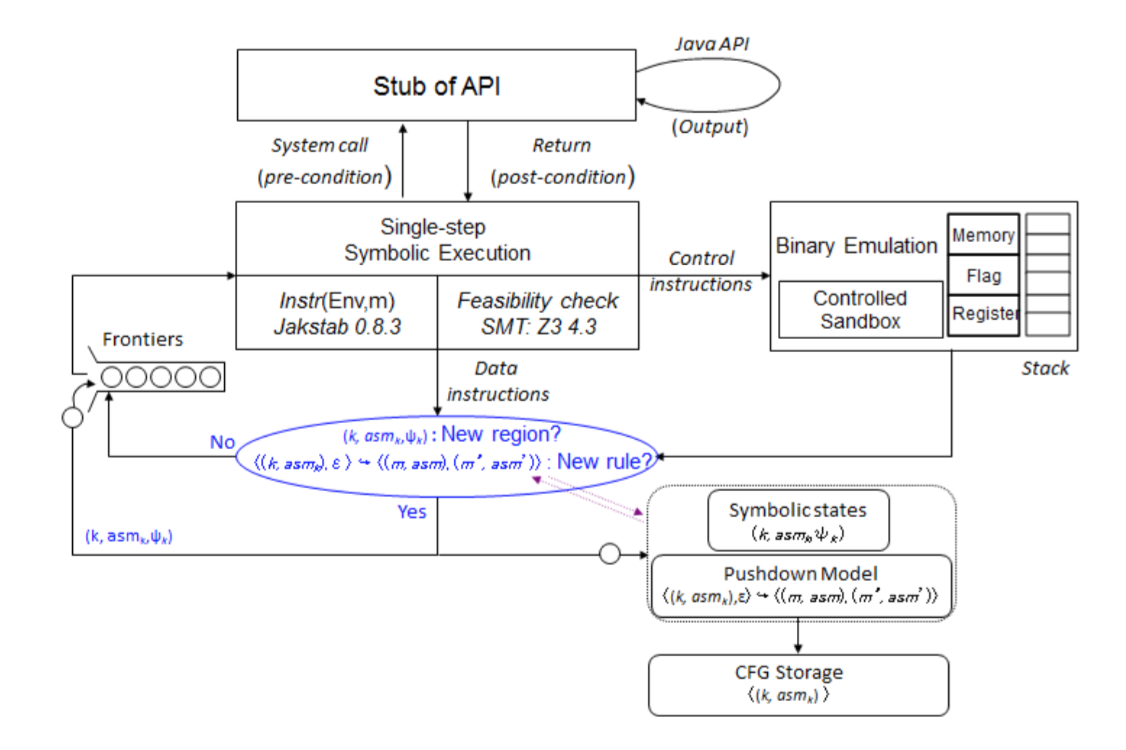
\includegraphics[width=0.7\textwidth]{bepum_architecture}
\caption{Kiến trúc của hệ thống BE-PUM}
\label{fig:BepumArchi}
\end{figure}

\hspace{0.5cm}Kiến trúc của hệ thống BE-PUM bao gồm 3 thành phần chính: symbolic execution, binary emulation và CFG storage. Hình \ref {fig:BepumArchi} mô tả kiến trúc của hệ thống BE-PUM. Trong đó, vai trò của các thành phần này như sau:

\begin{itemize}
\item{Single-step symbolic execution: sử dụng Jackstab để dịch ngược và chuyển đổi thành câu lệnh hợp ngữ tương ứng. Nếu câu lệnh hợp ngữ là câu lệnh chỉ tác động tới môi trường thực thi, cụ thể là các câu lệnh tính toán, câu lệnh ghi hoặc đọc trong bộ nhớ, bao gồm cả stack. Khi đó chỉ có môi trường thực thi được thay đổi và vị trí của câu lệnh tiếp theo chỉ được xác định bằng vị trí của câu lệnh hiện tại và kích thước câu lệnh. Nếu câu lệnh tiếp theo là câu lệnh điều khiển, cụ thể là các câu lệnh gọi hàm, câu lệnh trả về từ hàm, câu lệnh nhảy và câu lệnh nhảy có điều kiện, thì câu lệnh tiếp theo sẽ được tính toán thông qua dynamic symbolic execution.\\}
\item{
\begin{figure}[h]
\centering
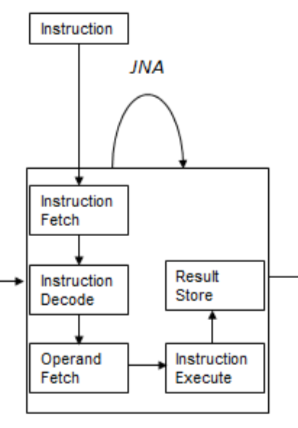
\includegraphics[width=0.3\textwidth]{bepum_binary_emulation}
\caption{Thành phần Binary Emulation trong BE-PUM}
\label{fig:BepumBE}
\end{figure}
Binary emulation: là thành phần quan trọng trong tổng thể kiến trúc của BE-PUM. Để có thể xử lý một câu lệnh hợp ngữ, hệ thống BE-PUM sẽ giả lập các thành phần của hệ thống, cụ thể là mô hình bộ nhớ của BE-PUM, mô hình này bao gồm tập 9 cờ được sử dụng trong hệ thống (AF, CF, DF, IF, OF, PF, SF, TF, và ZF), tập 20 thanh ghi (EAX, EBX, ECX, EDX, ESI, EDI, ESP, EBP, CS, DS, ES, FS, GS, SS, EIP, EFLAGS và 8 thanh ghi debug DRO, DR1, DR2, DR3, DR4, DR5, DR6, DR7, DR8), tập các giá trị bộ nhớ được lưu trữ trong đó một phần của bộ nhớ cho stack được giới hạn bởi thanh ghi esp và thanh ghi ebp. Bộ nhớ được giả lập trong BE-PUM được lưu trữ dưới dạng từng byte một. Ngoài việc giả lập câu lệnh hợp ngữ, thì API cũng được giả lập thông qua sử dụng Java Native Access cho phép gọi trực tiếp từ các thư viện liên kết động, trong đó giá trị trả về của các API sẽ được lưu trữ trong các thanh ghi tương ứng. Đối với các API đặc biệt tác động trực tiếp đến môi trường thực, một sandbox sẽ được xây dựng cho quá trình xử lý các API này. Ngoài ra, các API được sử dụng như một phần của kỹ thuật anti-reversing, anti-debugging, giá trị trả về sẽ là một giá trị symbolic. Hình \ref {fig:BepumBE} mô tả các quá trình xử lý một câu lệnh thực thi trong hệ thống BE-PUM.\\
}
\item{CFG storage: được sử dụng để lưu trữ một CFG node và CFG edge sau khi được tính toán chính xác. CFG storage sẽ được sử dụng để xây dựng mô hình quá trình thực thi cuối cùng của tập tin được phân tích.}
\end{itemize}

\subsection{Mô hình của BE-PUM}
\hspace{0.5cm}Kết quả của quá trình phân tích một tập tin thực thi là một mô hình quá trình thực thi, mô hình được sinh ra bởi hệ thống BE-PUM được biểu diễn dưới dạng Control Flow Graph hay CFG của chương trình.\\

\hspace{0.5cm}Một CFG là một tập của các node và edge. Trong đó một node của CFG bao gồm địa chỉ của câu lệnh và câu lệnh hợp ngữ tại địa chỉ đó, một edge của CFG là cạnh nối giữa 2 node của CFG.

\begin{code}
\begin{lstlisting}[captionpos=b,caption={Ví dụ về một đoạn mã thực thi},label={lst:SampleExe},frame=single]
00401000	pushl 0x00401007
00401005	jne 0x0040101A
0040100A 	movl fs:[0],esp			
\end{lstlisting}
\end{code}

\hspace{0.5cm}Với đoạn mã \ref {lst:SampleExe}, quá trình phân tích trên hệ thống BE-PUM sẽ sinh ra được mô hình của đoạn mã thực thi hay CFG của chương trình thực thi trên như sau:

\begin{figure}
\centering
\begin{tikzpicture}[shorten >=1pt,node distance=2cm,on grid,auto] 
   	\node[cfgstate,align=center](s_1){0x00401000\\\ pushl 0x00401007}; 
   	\node[cfgstate,align=center](s_2)[below of=s_1]{0x00401005\\\ jne 0x0040101A};
   	\node[cfgstate,align=center](s_3)[below of=s_2]{0x0040100A\\\ movl \%fs:[0],\%esp};
    \path[-{>[scale=2,length=3,width=3]}] 
    (s_1) edge node {} (s_2)
  	(s_2.east) edge [bend right=60] node {} (s_1.east)
    (s_2) edge node {} (s_3);	  
\end{tikzpicture}
\label{fig:SampleCFG}
\caption{CFG được sinh ra từ đoạn mã thực thi \ref {lst:SampleExe}}
\end{figure}

\subsection{Hạn chế của BE-PUM}

\hspace{0.5cm}Một số những hạn chế của hệ thống BE-PUM bao gồm:

\begin{itemize}
\item{Số lượng các câu lệnh hợp ngữ là rất lớn khoảng hơn 1000 câu lệnh và số lượng API là 4000. Tuy nhiên hiện tại BE-PUM chỉ hõ trợ được 200 câu lệnh và 400 API. Do đó đối với các malware hay packer sử dụng những câu lệnh hay API không được hỗ trợ, BE-PUM sẽ không thể phân tích tiếp tục được và do đó quá trình phân tích sẽ kết thúc.\\}
\item{Đối với những malware hay packer sử dụng những vòng lặp lớn hơn 1 tỷ lần thì quá trình phân tích trên BE-PUM sẽ kết thúc. Do đó khi gặp một vòng lặp với số lượng lớn thì quá trình phân tích sẽ tiếp tục được phân tích trên một đường thực thi khác.\\}
\item{Trong thực tế, trước khi thực thi tại entry point của chương trình, một số xử lý từ hệ điều hành sẽ được thực hiện qua đó tác động đến các giá trị thanh ghi, bộ nhớ và stack tại entry point. Do đó, khi quá trình phân tích bắt đầu, tại vị trí entry point, hệ thống BE-PUM sẽ mặc định thiết lập các giá trị mặc định cho stack bao gồm: địa chỉ chứa mã ASCII của tên tập tin, địa chỉ hàm xử lý exception của hệ thống, và giá trị trả về là một giá trị bất kì thuộc địa chỉ kernel.\\}
\item{Ngoài ra, các giá trị cờ cũng được thiết lập cụ thể như mô tả trong bảng \ref {table:BepumInitFlag}. Đối với các thanh ghi EAX, CS, DS, ES, FS, GS, SS, EFLAGS được thiết lập giá trị symbolic, các thanh ghi được thiết lập như mô tả trong bảng \ref {table:BepumInitReg}.
}
\end{itemize}

\begin{longtable}{ | m{2cm} | m{5cm} | }
\hline 
CF & False\\
\hline 
PF & True\\
\hline 
AF & False\\
\hline 
ZF & True\\
\hline 
SF & False\\
\hline 
TF & False\\
\hline 
DF & False\\
\hline 
OF & False\\
\hline 
IF & False\\
\hline
\caption{Các giá trị cờ được khởi tạo mặc định trong hệ thống BE-PUM}
\label{table:BepumInitFlag}
\end{longtable}

\begin{longtable}{ | m{5cm} | m{5cm} | }
\hline 
EIP, EDX & Địa chỉ entry point\\
\hline
ESP & Địa chỉ đỉnh của stack\\
\hline
EBP & Địa chỉ cơ sở của stack\\
\hline
ECX, EDI, ESI & 0\\
\hline
EBX & Địa chỉ PEB\\
\hline
\caption{Các giá trị thanh ghi được khởi tạo mặc định trong hệ thống BE-PUM}
\label{table:BepumInitReg}
\end{longtable}

\section{Model Checking và NuSMV}

\subsection{Model Checking}

\hspace{0.5cm}Model checking hay kiểm tra mô hình là một kỹ thuật tự động được sử dụng để kiểm tra một hệ thống tuần tự có số trạng thái hữu hạn bằng việc vét cạn toàn bộ không gian trạng thái của mô hình hệ thống. Bằng việc cung cấp một mô hình của hệ thống và một mô tả hành vi hệ thống cần kiểm tra dưới dạng biểu thức logic có yếu tố thời gian, phương pháp model checking có thể kết luận mô hình được kiểm tra có thoả mãn các tính chất được mô tả hay không. Hay nói một cách khác, với một mô hình hệ thống với số trạng thái hữu hạn $\mathcal{M}$ và một tính chất được biểu diễn dưới dạng hình thức $\phi$, phương pháp model checking sẽ kiểm tra nếu tính chất đó là thoả mãn với mô hình hệ thống: $\mathcal{M}\models\phi$. 

\subsection{Cấu trúc Kripke}

\hspace{0.5cm}Trong bước mô hình hoá được thực hiện trong phương pháp model checking sẽ chuyển đổi mô hình một hệ thống dưới dạng hình thức được sử dụng bởi một công cụ kiểm tra mô hình. Cấu trúc Kripke là một dạng của mô hình chuyển trạng thái biểu diễn hành vi của hệ thống trong suốt quá trình thời gian của hệ thống. Với AP là một tập của các mệnh đề nguyên tử, một cấu trúc Kripke trên tập AP $M = (S, S_0, R, L)$ được định nghĩa như sau:

\begin{itemize}
\item{$S$: tập hữu hạn các trạng thái.}
\item{$S_0 \subseteq S$: tập các trạng thái ban đầu.}
\item{$R \subseteq S \times S$: mối quan hệ chuyển trạng thái, theo đó với mọi trạng thái $s \in S$ luôn có trạng thái $s' \in S$ sao cho $R(s, s')$..}
\item{$L: S \rightarrow 2^{AP}$ là hàm xác định nhãn cho mỗi trạng thái với giá trị là các tập mệnh đề nguyên tử sao cho các mệnh đề đó là luôn đúng trong trạng thái đó.}
\end{itemize}

\begin{figure}
\centering
\begin{tikzpicture}[shorten >=1pt,node distance=3cm,on grid,auto] 
   	\node[state,initial](s_1){$\lbrace p,q\rbrace$}; 
   	\node[state](s_2)[below left=of s_1]{$\lbrace q\rbrace$};
   	\node[state](s_3)[below right=of s_2]{$\lbrace p\rbrace$};
    \path[-{>[scale=2,length=3,width=3]}] 
    (s_1) edge [bend left] node {} (s_2)
    (s_2) edge [bend left] node {} (s_1)
    	  edge node {} (s_3)
    (s_3) edge [loop above] node {} ();
\end{tikzpicture}
\caption{Ví dụ về cấu trúc Kripke}
\label{fig:KripkeStruct}
\end{figure}

\hspace{0.5cm}Với mô hình \ref {fig:KripkeStruct}, cho $AP = \lbrace p,q\rbrace$. Một cấu trúc Kripke $M = (S, S_0, R, L)$ được xác định với: $S = \lbrace s_1, s_2, s_3 \rbrace$, $S_0 = \lbrace s_1 \rbrace$, $R = \lbrace (s_1, s_2), (s_2, s_1), (s_2, s_3), (s_3, s_3)$ và $L = \lbrace (s_1,\lbrace p,q \rbrace), (s_2,\lbrace q \rbrace), (s_3,\lbrace p \rbrace) \rbrace$	 

\subsection{Logic có yếu tố thời gian}

\hspace{0.5cm}Logic yếu tố thời gian là mở rộng của logic mệnh đề truyền thống với việc kết hợp các toán tử mô tả được hành vi của hệ thống theo thời gian. Logic yếu tố thời gian cho phép mô tả được các tính chất của hệ thống thực như tính correctness, reachability, safety, liveness, fairness. Các toán tử được sự dụng để mô tả các hành vi của hệ thống theo thời gian là Path quantifiers và Temporal operators trong đó.

\begin{itemize}
\item{Path quantifiers: trong một biểu thức logic yếu tố thời gian được sử dụng để mô tả cấu trúc nhánh trong một cây tính toán. Trong đó 2 path quantifiers được sử dụng trong một biểu thức logic tính toán cây là $A$, mô tả với mọi đường tính toán, và $E$, mô tả tồn tại một đường tính toán.\\}
\item{Temporal operators: trong một biểu thức logic yếu tố thời gian được sử dụng để mô tả tính chất của một đường tính toán trong một cây tính toán. Trong đó 4 temporal operators được sử dụng trong một biểu thức tính toán cây là $X, F, G, U$.}
\end{itemize}

\hspace{0.5cm}\textbf{$X$("neXt")}: $X\varphi$ mô tả trạng thái tiếp theo trên một đường tính toán thoả mãn tính chất $\varphi$.
\begin{figure}
\centering
\begin{tikzpicture}[shorten >=1pt,node distance=2cm,on grid,auto] 
   	\node[state,initial,align=center,minimum size=0.5cm](s_0){$X\varphi$}; 
   	\node[state,align=center,minimum size=0.5cm,fill=gray](s_1)[right=of s_0]{$\varphi$};
   	\node[state,align=center,minimum size=0.5cm](s_2)[right=of s_1]{};
   	\node[state,align=center,minimum size=0.5cm](s_3)[right=of s_2]{};
   	\node (s_dots) [right=of s_3] {$\cdots$}; 
    \path[-{>[scale=2,length=3,width=3]}] 
    (s_0) edge node {} (s_1)
    (s_1) edge node {} (s_2)
    (s_2) edge node {} (s_3)
    (s_3) edge node {} (s_dots);
\end{tikzpicture}
\caption{Toán tử thời gian $X$}
\label{fig:nxtTemporal}
\end{figure}

\hspace{0.5cm}\textbf{$F$("Finally")}: $F\varphi$ mô tả một trạng thái bất kì trong tương lai thoả mãn tính chất $\varphi$.
\begin{figure}
\centering
\begin{tikzpicture}[shorten >=1pt,node distance=2cm,on grid,auto] 
   	\node[state,initial,align=center,minimum size=0.5cm](s_0){$F\varphi$}; 
   	\node[state,align=center,minimum size=0.5cm](s_1)[right=of s_0]{};
   	\node[state,align=center,minimum size=0.5cm](s_2)[right=of s_1]{};
   	\node[state,align=center,minimum size=0.5cm,fill=gray](s_3)[right=of s_2]{$\varphi$};
   	\node (s_dots) [right=of s_3] {$\cdots$}; 
    \path[-{>[scale=2,length=3,width=3]}] 
    (s_0) edge node {} (s_1)
    (s_1) edge node {} (s_2)
    (s_2) edge node {} (s_3)
    (s_3) edge node {} (s_dots);
\end{tikzpicture}
\caption{Toán tử thời gian $F$}
\label{fig:futureTemporal}
\end{figure}

\hspace{0.5cm}\textbf{$G$("Globally")}: $G\varphi$ mô tả tất cả trạng thái trong tương lai thoả mãn tính chất $\varphi$.
\begin{figure}
\centering
\begin{tikzpicture}[shorten >=1pt,node distance=2cm,on grid,auto] 
   	\node[state,initial,align=center,minimum size=0.5cm,fill=gray](s_0){$G\varphi,\varphi$}; 
   	\node[state,align=center,minimum size=0.5cm,fill=gray](s_1)[right=of s_0]{$\varphi$};
   	\node[state,align=center,minimum size=0.5cm,fill=gray](s_2)[right=of s_1]{$\varphi$};
   	\node[state,align=center,minimum size=0.5cm,fill=gray](s_3)[right=of s_2]{$\varphi$};
   	\node (s_dots) [right=of s_3] {$\cdots$}; 
    \path[-{>[scale=2,length=3,width=3]}] 
    (s_0) edge node {} (s_1)
    (s_1) edge node {} (s_2)
    (s_2) edge node {} (s_3)
    (s_3) edge node {} (s_dots);
\end{tikzpicture}
\caption{Toán tử thời gian $G$}
\label{fig:globalTemporal}
\end{figure}


\hspace{0.5cm}\textbf{$U$("Until")}: $\varphi_1U\varphi_2$ mô tả tính chất $\varphi_1$ thoả mãn trên tất cả trạng thái cho đến khi tính chất $\varphi_2$ thoả mãn.
\begin{figure}
\centering
\begin{tikzpicture}[shorten >=1pt,node distance=2cm,on grid,auto] 
   	\node[state,initial,align=center,minimum size=0.5cm,fill=white!30!gray](s_0){$\varphi_1 U \varphi_2,\varphi_1$}; 
   	\node[state,align=center,minimum size=0.5cm,fill=white!30!gray](s_1)[right=of s_0]{$\varphi_1$};
   	\node[state,align=center,minimum size=0.5cm,fill=white!30!gray](s_2)[right=of s_1]{$\varphi_1$};
   	\node[state,align=center,minimum size=0.5cm,fill=gray](s_3)[right=of s_2]{$\varphi_2$};
   	\node (s_dots) [right=of s_3] {$\cdots$}; 
    \path[-{>[scale=2,length=3,width=3]}] 
    (s_0) edge node {} (s_1)
    (s_1) edge node {} (s_2)
    (s_2) edge node {} (s_3)
    (s_3) edge node {} (s_dots);
\end{tikzpicture}
\end{figure}

\subsection{CTL}

\hspace{0.5cm}\textbf{Syntax}
\begin{code}
\begin{lstlisting}[captionpos=b,caption={CTL Syntax},label={lst:CTLSyntax},frame=single,mathescape=true]
$\Phi \Coloneqq true\;|\;p\;|\;(\neg\Phi)\;|\;(\Phi_1\wedge\Phi_2)\;|\;A\phi\;|\;E\phi$
$\phi \Coloneqq X\Phi\;|\;\Phi_1 U\Phi_2$
\end{lstlisting}
\end{code}

\hspace{0.5cm}\textbf{Semantic}
\begin{center}
\resizebox{10cm}{!}{
\begin{tikzpicture}[shorten >=1pt,node distance=1.5cm,on grid,auto] 
   	\node[state,initial,minimum size=0.5cm](s_1){}; 
   	\node[state, minimum size=0.5cm][below=of s_1](s_3){};
   	\node[state, minimum size=0.5cm][left=4cm of s_3](s_2){};
   	\node[state, minimum size=0.5cm][right=4cm of s_3,fill=red](s_4){};
   	\node[state, minimum size=0.5cm][below left=of s_2](s_5){};
   	\node[state, minimum size=0.5cm][below right=of s_2](s_6){};
   	\node[state, minimum size=0.5cm][below=1.06cm of s_3](s_7){};
   	\node[state, minimum size=0.5cm][below left=of s_4](s_8){};
	\node[state, minimum size=0.5cm][below right=of s_4](s_9){};
	\node[state, minimum size=0.5cm][below=1.2cm of s_5](s_10){};
	\node[state, minimum size=0.5cm][below left=1.7cm of s_7](s_11){};
	\node[state, minimum size=0.5cm][below right=1.7cm of s_7](s_12){};
	\node[state, minimum size=0.5cm][below=1.2cm of s_9](s_13){};
	\node[minimum size=0.5cm][below=of s_10](s_14){$\cdots$};
	\node[minimum size=0.5cm][below=of s_6](s_15){$\cdots$};
	\node[state, minimum size=0.5cm][below=of s_11](s_16){};
	\node[minimum size=0.5cm][below=of s_12](s_17){$\cdots$};
	\node[minimum size=0.5cm][below=of s_8](s_18){$\cdots$};
	\node[state,minimum size=0.5cm][below=of s_13](s_19){};
	\node[state,minimum size=0.5cm][below left=2.12cm of s_13](s_20){};
	\node[state,minimum size=0.5cm][below right=2.12cm of s_13](s_21){};
	\node[minimum size=0.5cm][below=of s_16](s_22){$\cdots$};
	\node[minimum size=0.5cm][below=of s_19](s_23){$\cdots$};
	\node[minimum size=0.5cm][below=of s_20](s_24){$\cdots$};
	\node[minimum size=0.5cm][below=of s_21](s_25){$\cdots$};
    \path[-{>[scale=2,length=3,width=3]}] 
    (s_1) edge node {} (s_2)
    	edge node {} (s_3)
    	edge node {} (s_4)
    (s_2) edge node {} (s_5)
    	edge node {} (s_6)
    (s_3) edge node {} (s_7)
    (s_4) edge node {} (s_8)
    	edge node {} (s_9)
    (s_5) edge node {} (s_10)
    (s_7) edge node {} (s_11)
    	edge node {} (s_12)
    (s_9) edge node {} (s_13)
    (s_11) edge node {} (s_16)
    (s_13) edge node {} (s_19)
    	edge node {} (s_20)
    	edge node {} (s_21);
\end{tikzpicture}
}\\
$M,s_0\models EX$\color{red}p
\end{center}

\begin{center}
\resizebox{10cm}{!}{
\begin{tikzpicture}[shorten >=1pt,node distance=1.5cm,on grid,auto] 
   	\node[state,initial,minimum size=0.5cm,fill=red](s_1){}; 
   	\node[state, minimum size=0.5cm][below=of s_1,fill=red](s_3){};
   	\node[state, minimum size=0.5cm][left=4cm of s_3](s_2){};
   	\node[state, minimum size=0.5cm][right=4cm of s_3](s_4){};
   	\node[state, minimum size=0.5cm][below left=of s_2](s_5){};
   	\node[state, minimum size=0.5cm][below right=of s_2](s_6){};
   	\node[state, minimum size=0.5cm][below=1.06cm of s_3,fill=red](s_7){};
   	\node[state, minimum size=0.5cm][below left=of s_4](s_8){};
	\node[state, minimum size=0.5cm][below right=of s_4](s_9){};
	\node[state, minimum size=0.5cm][below=1.2cm of s_5](s_10){};
	\node[state, minimum size=0.5cm][below left=1.7cm of s_7,fill=red](s_11){};
	\node[state, minimum size=0.5cm][below right=1.7cm of s_7](s_12){};
	\node[state, minimum size=0.5cm][below=1.2cm of s_9](s_13){};
	\node[minimum size=0.5cm][below=of s_10](s_14){$\cdots$};
	\node[minimum size=0.5cm][below=of s_6](s_15){$\cdots$};
	\node[state, minimum size=0.5cm][below=of s_11,fill=red](s_16){};
	\node[minimum size=0.5cm][below=of s_12](s_17){$\cdots$};
	\node[minimum size=0.5cm][below=of s_8](s_18){$\cdots$};
	\node[state,minimum size=0.5cm][below=of s_13](s_19){};
	\node[state,minimum size=0.5cm][below left=2.12cm of s_13](s_20){};
	\node[state,minimum size=0.5cm][below right=2.12cm of s_13](s_21){};
	\node[minimum size=0.5cm][below=of s_16](s_22){$\cdots$};
	\node[minimum size=0.5cm][below=of s_19](s_23){$\cdots$};
	\node[minimum size=0.5cm][below=of s_20](s_24){$\cdots$};
	\node[minimum size=0.5cm][below=of s_21](s_25){$\cdots$};
    \path[-{>[scale=2,length=3,width=3]}] 
    (s_1) edge node {} (s_2)
    	edge node {} (s_3)
    	edge node {} (s_4)
    (s_2) edge node {} (s_5)
    	edge node {} (s_6)
    (s_3) edge node {} (s_7)
    (s_4) edge node {} (s_8)
    	edge node {} (s_9)
    (s_5) edge node {} (s_10)
    (s_7) edge node {} (s_11)
    	edge node {} (s_12)
    (s_9) edge node {} (s_13)
    (s_11) edge node {} (s_16)
    (s_13) edge node {} (s_19)
    	edge node {} (s_20)
    	edge node {} (s_21);
\end{tikzpicture}
}\\
$M,s_0\models EG$\color{red}p
\end{center}

\begin{center}
\resizebox{10cm}{!}{
\begin{tikzpicture}[shorten >=1pt,node distance=1.5cm,on grid,auto] 
   	\node[state,initial,minimum size=0.5cm,fill=red](s_1){}; 
   	\node[state, minimum size=0.5cm][below=of s_1](s_3){};
   	\node[state, minimum size=0.5cm][left=4cm of s_3](s_2){};
   	\node[state, minimum size=0.5cm][right=4cm of s_3,fill=red](s_4){};
   	\node[state, minimum size=0.5cm][below left=of s_2](s_5){};
   	\node[state, minimum size=0.5cm][below right=of s_2](s_6){};
   	\node[state, minimum size=0.5cm][below=1.06cm of s_3](s_7){};
   	\node[state, minimum size=0.5cm][below left=of s_4](s_8){};
	\node[state, minimum size=0.5cm][below right=of s_4,fill=red](s_9){};
	\node[state, minimum size=0.5cm][below=1.2cm of s_5](s_10){};
	\node[state, minimum size=0.5cm][below left=1.7cm of s_7](s_11){};
	\node[state, minimum size=0.5cm][below right=1.7cm of s_7](s_12){};
	\node[state, minimum size=0.5cm][below=1.2cm of s_9,fill=red](s_13){};
	\node[minimum size=0.5cm][below=of s_10](s_14){$\cdots$};
	\node[minimum size=0.5cm][below=of s_6](s_15){$\cdots$};
	\node[state, minimum size=0.5cm][below=of s_11](s_16){};
	\node[minimum size=0.5cm][below=of s_12](s_17){$\cdots$};
	\node[minimum size=0.5cm][below=of s_8](s_18){$\cdots$};
	\node[state,minimum size=0.5cm][below=of s_13](s_19){};
	\node[state,minimum size=0.5cm][below left=2.12cm of s_13,fill=blue](s_20){};
	\node[state,minimum size=0.5cm][below right=2.12cm of s_13](s_21){};
	\node[minimum size=0.5cm][below=of s_16](s_22){$\cdots$};
	\node[minimum size=0.5cm][below=of s_19](s_23){$\cdots$};
	\node[minimum size=0.5cm][below=of s_20](s_24){$\cdots$};
	\node[minimum size=0.5cm][below=of s_21](s_25){$\cdots$};
    \path[-{>[scale=2,length=3,width=3]}] 
    (s_1) edge node {} (s_2)
    	edge node {} (s_3)
    	edge node {} (s_4)
    (s_2) edge node {} (s_5)
    	edge node {} (s_6)
    (s_3) edge node {} (s_7)
    (s_4) edge node {} (s_8)
    	edge node {} (s_9)
    (s_5) edge node {} (s_10)
    (s_7) edge node {} (s_11)
    	edge node {} (s_12)
    (s_9) edge node {} (s_13)
    (s_11) edge node {} (s_16)
    (s_13) edge node {} (s_19)
    	edge node {} (s_20)
    	edge node {} (s_21);
\end{tikzpicture}
}\\
$M,s_0\models E$\color{red}q$\;U\;$\color{blue}p
\end{center}

\begin{center}
\resizebox{10cm}{!}{
\begin{tikzpicture}[shorten >=1pt,node distance=1.5cm,on grid,auto] 
   	\node[state,initial,minimum size=0.5cm](s_1){}; 
   	\node[state, minimum size=0.5cm][below=of s_1](s_3){};
   	\node[state, minimum size=0.5cm][left=4cm of s_3](s_2){};
   	\node[state, minimum size=0.5cm][right=4cm of s_3](s_4){};
   	\node[state, minimum size=0.5cm][below left=of s_2](s_5){};
   	\node[state, minimum size=0.5cm][below right=of s_2,fill=red](s_6){};
   	\node[state, minimum size=0.5cm][below=1.06cm of s_3](s_7){};
   	\node[state, minimum size=0.5cm][below left=of s_4](s_8){};
	\node[state, minimum size=0.5cm][below right=of s_4](s_9){};
	\node[state, minimum size=0.5cm][below=1.2cm of s_5](s_10){};
	\node[state, minimum size=0.5cm][below left=1.7cm of s_7](s_11){};
	\node[state, minimum size=0.5cm][below right=1.7cm of s_7](s_12){};
	\node[state, minimum size=0.5cm][below=1.2cm of s_9](s_13){};
	\node[minimum size=0.5cm][below=of s_10](s_14){$\cdots$};
	\node[minimum size=0.5cm][below=of s_6](s_15){$\cdots$};
	\node[state, minimum size=0.5cm][below=of s_11](s_16){};
	\node[minimum size=0.5cm][below=of s_12](s_17){$\cdots$};
	\node[minimum size=0.5cm][below=of s_8](s_18){$\cdots$};
	\node[state,minimum size=0.5cm][below=of s_13](s_19){};
	\node[state,minimum size=0.5cm][below left=2.12cm of s_13](s_20){};
	\node[state,minimum size=0.5cm][below right=2.12cm of s_13](s_21){};
	\node[minimum size=0.5cm][below=of s_16](s_22){$\cdots$};
	\node[minimum size=0.5cm][below=of s_19](s_23){$\cdots$};
	\node[minimum size=0.5cm][below=of s_20](s_24){$\cdots$};
	\node[minimum size=0.5cm][below=of s_21](s_25){$\cdots$};
    \path[-{>[scale=2,length=3,width=3]}] 
    (s_1) edge node {} (s_2)
    	edge node {} (s_3)
    	edge node {} (s_4)
    (s_2) edge node {} (s_5)
    	edge node {} (s_6)
    (s_3) edge node {} (s_7)
    (s_4) edge node {} (s_8)
    	edge node {} (s_9)
    (s_5) edge node {} (s_10)
    (s_7) edge node {} (s_11)
    	edge node {} (s_12)
    (s_9) edge node {} (s_13)
    (s_11) edge node {} (s_16)
    (s_13) edge node {} (s_19)
    	edge node {} (s_20)
    	edge node {} (s_21);
\end{tikzpicture}
}\\
$M,s_0\models EF$\color{red}p
\end{center}

\begin{center}
\resizebox{10cm}{!}{
\begin{tikzpicture}[shorten >=1pt,node distance=1.5cm,on grid,auto] 
   	\node[state,initial,minimum size=0.5cm](s_1){}; 
   	\node[state, minimum size=0.5cm][below=of s_1,fill=red](s_3){};
   	\node[state, minimum size=0.5cm][left=4cm of s_3,fill=red](s_2){};
   	\node[state, minimum size=0.5cm][right=4cm of s_3,fill=red](s_4){};
   	\node[state, minimum size=0.5cm][below left=of s_2](s_5){};
   	\node[state, minimum size=0.5cm][below right=of s_2](s_6){};
   	\node[state, minimum size=0.5cm][below=1.06cm of s_3](s_7){};
   	\node[state, minimum size=0.5cm][below left=of s_4](s_8){};
	\node[state, minimum size=0.5cm][below right=of s_4](s_9){};
	\node[state, minimum size=0.5cm][below=1.2cm of s_5](s_10){};
	\node[state, minimum size=0.5cm][below left=1.7cm of s_7](s_11){};
	\node[state, minimum size=0.5cm][below right=1.7cm of s_7](s_12){};
	\node[state, minimum size=0.5cm][below=1.2cm of s_9](s_13){};
	\node[minimum size=0.5cm][below=of s_10](s_14){$\cdots$};
	\node[minimum size=0.5cm][below=of s_6](s_15){$\cdots$};
	\node[state, minimum size=0.5cm][below=of s_11](s_16){};
	\node[minimum size=0.5cm][below=of s_12](s_17){$\cdots$};
	\node[minimum size=0.5cm][below=of s_8](s_18){$\cdots$};
	\node[state,minimum size=0.5cm][below=of s_13](s_19){};
	\node[state,minimum size=0.5cm][below left=2.12cm of s_13](s_20){};
	\node[state,minimum size=0.5cm][below right=2.12cm of s_13](s_21){};
	\node[minimum size=0.5cm][below=of s_16](s_22){$\cdots$};
	\node[minimum size=0.5cm][below=of s_19](s_23){$\cdots$};
	\node[minimum size=0.5cm][below=of s_20](s_24){$\cdots$};
	\node[minimum size=0.5cm][below=of s_21](s_25){$\cdots$};
    \path[-{>[scale=2,length=3,width=3]}] 
    (s_1) edge node {} (s_2)
    	edge node {} (s_3)
    	edge node {} (s_4)
    (s_2) edge node {} (s_5)
    	edge node {} (s_6)
    (s_3) edge node {} (s_7)
    (s_4) edge node {} (s_8)
    	edge node {} (s_9)
    (s_5) edge node {} (s_10)
    (s_7) edge node {} (s_11)
    	edge node {} (s_12)
    (s_9) edge node {} (s_13)
    (s_11) edge node {} (s_16)
    (s_13) edge node {} (s_19)
    	edge node {} (s_20)
    	edge node {} (s_21);
\end{tikzpicture}
}\\
$M,s_0\models AX$\color{red}p
\end{center}

\begin{center}
\resizebox{10cm}{!}{
\begin{tikzpicture}[shorten >=1pt,node distance=1.5cm,on grid,auto] 
   	\node[state,initial,minimum size=0.5cm,fill=red](s_1){}; 
   	\node[state, minimum size=0.5cm][below=of s_1,fill=red](s_3){};
   	\node[state, minimum size=0.5cm][left=4cm of s_3,fill=red](s_2){};
   	\node[state, minimum size=0.5cm][right=4cm of s_3,fill=red](s_4){};
   	\node[state, minimum size=0.5cm][below left=of s_2,fill=red](s_5){};
   	\node[state, minimum size=0.5cm][below right=of s_2,fill=red](s_6){};
   	\node[state, minimum size=0.5cm][below=1.06cm of s_3,fill=red](s_7){};
   	\node[state, minimum size=0.5cm][below left=of s_4,fill=red](s_8){};
	\node[state, minimum size=0.5cm][below right=of s_4,fill=red](s_9){};
	\node[state, minimum size=0.5cm][below=1.2cm of s_5,fill=red](s_10){};
	\node[state, minimum size=0.5cm][below left=1.7cm of s_7,fill=red](s_11){};
	\node[state, minimum size=0.5cm][below right=1.7cm of s_7,fill=red](s_12){};
	\node[state, minimum size=0.5cm][below=1.2cm of s_9,fill=red](s_13){};
	\node[minimum size=0.5cm][below=of s_10](s_14){$\cdots$};
	\node[minimum size=0.5cm][below=of s_6](s_15){$\cdots$};
	\node[state, minimum size=0.5cm][below=of s_11,fill=red](s_16){};
	\node[minimum size=0.5cm][below=of s_12](s_17){$\cdots$};
	\node[minimum size=0.5cm][below=of s_8](s_18){$\cdots$};
	\node[state,minimum size=0.5cm][below=of s_13,fill=red](s_19){};
	\node[state,minimum size=0.5cm][below left=2.12cm of s_13,fill=red](s_20){};
	\node[state,minimum size=0.5cm][below right=2.12cm of s_13,fill=red](s_21){};
	\node[minimum size=0.5cm][below=of s_16](s_22){$\cdots$};
	\node[minimum size=0.5cm][below=of s_19](s_23){$\cdots$};
	\node[minimum size=0.5cm][below=of s_20](s_24){$\cdots$};
	\node[minimum size=0.5cm][below=of s_21](s_25){$\cdots$};
    \path[-{>[scale=2,length=3,width=3]}] 
    (s_1) edge node {} (s_2)
    	edge node {} (s_3)
    	edge node {} (s_4)
    (s_2) edge node {} (s_5)
    	edge node {} (s_6)
    (s_3) edge node {} (s_7)
    (s_4) edge node {} (s_8)
    	edge node {} (s_9)
    (s_5) edge node {} (s_10)
    (s_7) edge node {} (s_11)
    	edge node {} (s_12)
    (s_9) edge node {} (s_13)
    (s_11) edge node {} (s_16)
    (s_13) edge node {} (s_19)
    	edge node {} (s_20)
    	edge node {} (s_21);
\end{tikzpicture}
}\\
$M,s_0\models AG$\color{red}p
\end{center}

\begin{center}
\resizebox{10cm}{!}{
\begin{tikzpicture}[shorten >=1pt,node distance=1.5cm,on grid,auto] 
   	\node[state,initial,minimum size=0.5cm](s_1){}; 
   	\node[state, minimum size=0.5cm][below=of s_1](s_3){};
   	\node[state, minimum size=0.5cm][left=4cm of s_3](s_2){};
   	\node[state, minimum size=0.5cm][right=4cm of s_3](s_4){};
   	\node[state, minimum size=0.5cm][below left=of s_2](s_5){};
   	\node[state, minimum size=0.5cm][below right=of s_2,fill=red](s_6){};
   	\node[state, minimum size=0.5cm][below=1.06cm of s_3](s_7){};
   	\node[state, minimum size=0.5cm][below left=of s_4,fill=red](s_8){};
	\node[state, minimum size=0.5cm][below right=of s_4](s_9){};
	\node[state, minimum size=0.5cm][below=1.2cm of s_5,fill=red](s_10){};
	\node[state, minimum size=0.5cm][below left=1.7cm of s_7](s_11){};
	\node[state, minimum size=0.5cm][below right=1.7cm of s_7,fill=red](s_12){};
	\node[state, minimum size=0.5cm][below=1.2cm of s_9,fill=red](s_13){};
	\node[minimum size=0.5cm][below=of s_10](s_14){$\cdots$};
	\node[minimum size=0.5cm][below=of s_6](s_15){$\cdots$};
	\node[state, minimum size=0.5cm][below=of s_11,fill=red](s_16){};
	\node[minimum size=0.5cm][below=of s_12](s_17){$\cdots$};
	\node[minimum size=0.5cm][below=of s_8](s_18){$\cdots$};
	\node[state,minimum size=0.5cm][below=of s_13](s_19){};
	\node[state,minimum size=0.5cm][below left=2.12cm of s_13](s_20){};
	\node[state,minimum size=0.5cm][below right=2.12cm of s_13](s_21){};
	\node[minimum size=0.5cm][below=of s_16](s_22){$\cdots$};
	\node[minimum size=0.5cm][below=of s_19](s_23){$\cdots$};
	\node[minimum size=0.5cm][below=of s_20](s_24){$\cdots$};
	\node[minimum size=0.5cm][below=of s_21](s_25){$\cdots$};
    \path[-{>[scale=2,length=3,width=3]}] 
    (s_1) edge node {} (s_2)
    	edge node {} (s_3)
    	edge node {} (s_4)
    (s_2) edge node {} (s_5)
    	edge node {} (s_6)
    (s_3) edge node {} (s_7)
    (s_4) edge node {} (s_8)
    	edge node {} (s_9)
    (s_5) edge node {} (s_10)
    (s_7) edge node {} (s_11)
    	edge node {} (s_12)
    (s_9) edge node {} (s_13)
    (s_11) edge node {} (s_16)
    (s_13) edge node {} (s_19)
    	edge node {} (s_20)
    	edge node {} (s_21);
\end{tikzpicture}
}\\
$M,s_0\models AF$\color{red}p
\end{center}

\begin{center}
\resizebox{10cm}{!}{
\begin{tikzpicture}[shorten >=1pt,node distance=1.5cm,on grid,auto] 
   	\node[state,initial,minimum size=0.5cm,fill=red](s_1){}; 
   	\node[state, minimum size=0.5cm][below=of s_1,fill=red](s_3){};
   	\node[state, minimum size=0.5cm][left=4cm of s_3,fill=red](s_2){};
   	\node[state, minimum size=0.5cm][right=4cm of s_3,fill=red](s_4){};
   	\node[state, minimum size=0.5cm][below left=of s_2,fill=red](s_5){};
   	\node[state, minimum size=0.5cm][below right=of s_2,fill=blue](s_6){};
   	\node[state, minimum size=0.5cm][below=1.06cm of s_3,fill=red](s_7){};
   	\node[state, minimum size=0.5cm][below left=of s_4,fill=blue](s_8){};
	\node[state, minimum size=0.5cm][below right=of s_4,fill=red](s_9){};
	\node[state, minimum size=0.5cm][below=1.2cm of s_5,fill=blue](s_10){};
	\node[state, minimum size=0.5cm][below left=1.7cm of s_7,fill=red](s_11){};
	\node[state, minimum size=0.5cm][below right=1.7cm of s_7,fill=blue](s_12){};
	\node[state, minimum size=0.5cm][below=1.2cm of s_9,fill=blue](s_13){};
	\node[minimum size=0.5cm][below=of s_10](s_14){$\cdots$};
	\node[minimum size=0.5cm][below=of s_6](s_15){$\cdots$};
	\node[state, minimum size=0.5cm][below=of s_11,fill=blue](s_16){};
	\node[minimum size=0.5cm][below=of s_12](s_17){$\cdots$};
	\node[minimum size=0.5cm][below=of s_8](s_18){$\cdots$};
	\node[state,minimum size=0.5cm][below=of s_13](s_19){};
	\node[state,minimum size=0.5cm][below left=2.12cm of s_13](s_20){};
	\node[state,minimum size=0.5cm][below right=2.12cm of s_13](s_21){};
	\node[minimum size=0.5cm][below=of s_16](s_22){$\cdots$};
	\node[minimum size=0.5cm][below=of s_19](s_23){$\cdots$};
	\node[minimum size=0.5cm][below=of s_20](s_24){$\cdots$};
	\node[minimum size=0.5cm][below=of s_21](s_25){$\cdots$};
    \path[-{>[scale=2,length=3,width=3]}] 
    (s_1) edge node {} (s_2)
    	edge node {} (s_3)
    	edge node {} (s_4)
    (s_2) edge node {} (s_5)
    	edge node {} (s_6)
    (s_3) edge node {} (s_7)
    (s_4) edge node {} (s_8)
    	edge node {} (s_9)
    (s_5) edge node {} (s_10)
    (s_7) edge node {} (s_11)
    	edge node {} (s_12)
    (s_9) edge node {} (s_13)
    (s_11) edge node {} (s_16)
    (s_13) edge node {} (s_19)
    	edge node {} (s_20)
    	edge node {} (s_21);
\end{tikzpicture}
}\\
$M,s_0\models A$\color{red}q$\;U\;$\color{blue}p
\end{center}

\subsection{Kiểm tra mô hình với NuSMV}

\hspace{0.5cm}Công cụ kiểm tra mô hình NuSMV được sử dụng để kiểm tra một mô hình có thoã mãn tính chất cần được kiểm tra hay không. Trong đó, mô hình cần kiểm tra sẽ được chuyển đổi qua mô hình NuSMV sử dụng ngôn ngữ SMV và tính chất cần được mô tả hình thức dưới dạng biểu thức logic CTL hoặc LTL.\\

\hspace{0.5cm}Ví dụ \ref {lst:NuSMVSample} sẽ trình bày cú pháp đơn giản để xây dựng một mô hình NuSMV, qua đó chuyển đổi một mô hình cơ bản quá trình thực thi của một tập tin tương ứng với mô hình \ref {lst:SampleExe} đã được trình bày ở trên, dưới dạng mô hình NuSMV. Cũng như sẽ mô tả một tính chất đơn giản để thực hiện việc kiểm tra trên mô hình này, giả sử tính chất cần được kiểm tra là: "Tồn tại một câu lệnh push một giá trị bất kì vào stack trong quá trình thực thi."

\begin{code}
\begin{lstlisting}[captionpos=b,caption={Ví dụ về kiểm tra mô hình trên NuSMV},label={lst:NuSMVSample},frame=single]

MODULE operand2(addr)
VAR
  op:{esp, undefined}
ASSIGN
  init(op):=undefined;
  next(op):=
    case
      (addr=0x00401000):undefined;
      (addr=0x00401005):{esp, undefined};
      TRUE: undefined;
    esac;

MODULE operand1(addr)
VAR
  op:{0x00401007, 0x0040101A, fs:[0], undefined}
ASSIGN
  init(op):=0x00401007;
  next(op):=
    case
      (addr=0x00401000):0x0040101A;
      (addr=0x00401005):{fs:[0], 0x00401007};
      TRUE: undefined;
    esac;

MODULE mnemonic(addr)
VAR
  mnem:{pushl, jne, movl, undefined}
ASSIGN
  init(mnem):=pushl;
  next(mnem):=
    case
      (addr=0x00401000):jne;
      (addr=0x00401005):{movl, pushl};
      TRUE: undefined;
    esac;

MODULE state
VAR
  addr:{0x00401000,0x00401005,0x0040100A};
  mnem:mnemonic(addr);
  op1:operand1(addr);
  op2:operand2(addr);
ASSIGN
  init(addr):=0x00401000;
  next(addr):=
    case
      (addr=0x00401000):0x00401005;
      (addr=0x00401005):{0x0040100A, 0x00401000};
      TRUE: addr;
    esac;

MODULE main
VAR
  s: state;

CTLSPEC AF(s.mnem == pushl)

\end{lstlisting}
\end{code}

\section{Các kỹ thuật chính của Packer}

\hspace{0.5cm}Hiện tại, hệ thống BE-PUM đã phân tích hoàn toàn được 27 packer. Các kỹ thuật trong 27 packer này được chia thành 6 nhóm bao gồm:

\begin{itemize}
\item{Code placing obfuscation: Dynamic Code và Code layout}
\item{Self-modification code: Dynamic code}
\item{Instruction Obfuscation: Indirect Jump}
\item{Anti-tracing: Structured Exception Handler và 2 Special APIs}
\item{Arithmetic Operation: Obfuscated constants và Checksumming}
\item{Anti-tampering: Checksumming, Timing check, Anti-debugging, Anti-rewriting và Hardware breakpoints}
\end{itemize}

\subsection{Code placing obfuscation}
\begin{enumerate}
\item{Dynamic Code: nhóm kỹ thuật Dynamic code được sử dụng trong packer dưới dạng 2 kỹ thuật chính là Code overwriting và kỹ thuật Packing/unpacking.  
\begin{itemize}
\item{Code Overwriting: kỹ thuật này còn được gọi là kỹ thuật Self-modifying code (SMC). Theo đó, packer sẽ sử dụng kỹ thuật này để có thể thay đổi động mã nhị phân của chương trình trong quá trình thực thi, chính vì giá trị này hay giá trị opcode thay đổi dẫn đến câu lệnh tại địa chỉ đó cũng được thay đổi. Packer sử dụng kỹ thuật này để có thể thay đổi chữ ký của mình vì thế đối với những phần mềm chống malware nhận dạng packer thông qua chữ ký sẽ không thể nhận dạng được vì chữ ký này luôn thay đổi liên tục. Chính vì hệ thống BE-PUM hỗ trợ giải thuật On-the-fly model generation với khả năng xử lý những thay động trong mã nhị phân mà hệ thống BE-PUM dễ dàng xử lý được kỹ thuật này. Đoạn mã \ref {lst:SMCinYODA} mô tả kỹ thuật Code overwriting được sử dụng trong packer YODA. Theo đó sau khi thực thi đoạn mã tại vị trí 0x004040C6 với giá trị EDI = 0x004040C6, câu lệnh CMP đã được thay đổi thành câu lệnh MOV. 
\begin{code}
\begin{lstlisting}[captionpos=b,caption={Kỹ thuật Code Overwriting sử dụng trong packer YODA},label={lst:SMCinYODA},frame=single]
4040C3	STOS BYTE PTR ES:[EDI]
4040C6	CMP ECX, EBP

4040C3	STOS BYTE PTR ES:[EDI]
4040C6	MOV EBP, ECX
\end{lstlisting}
\end{code}
}
\item{Packing/Unpacking: kỹ thuật này còn được gọi là kỹ thuật Encryption/Decryption, lõi của kỹ thuật này chính là kỹ thuật SMC đã được trình bày như trên, với số lượng vòng lặp được sử dụng để thay đổi một hoặc nhiều byte dẫn đến việc thay đổi câu lệnh liên tục trong suốt quá trình thực thi. Chính vì hệ thống BE-PUM có thể xử lý kỹ thuật SMC và hỗ trợ Dynamic symbolic execution mà giải thuật này dễ dàng được xử lý. Đoạn mã \ref {lst:PUinYODA} mô tả kỹ thuật packing/unpacking được sử dụng trong packer YODA.  
\begin{code}
\begin{lstlisting}[captionpos=b,caption={Kỹ thuật Packing/unpacking sử dụng trong packer YODA},label={lst:PUinYODA},frame=single]
404092	LODS BYTE PTR DS:[EDI]
404093	ROR AL, 0DB
404096	JMP 404099
404099	DEC AL
40409B	ADD AL,21
40409D	DEC AL
40409F	ADD AL,CL
4040A1	STC
4040A2	ADD AL,57
4040A4	CLC
4040A5	ADD AL,8A
4040A7	STC
4040A8	NOP
4040A9	ROR AL,0D7
4040AC	ROR AL,10
4040AF	JMP 4040B2
4040B2	ROR AL,5B
4040B5	CLC
4040B6	XOR AL,0D6
4040B8	STC
4040B9	XOR AL,0D4
4040BB	SUB AL,CL
4040BD	JMP 4040C0 
4040C0	SUB AL,8B
4040C2	CLC		
4040C3	STOS BYTE PTR ES:[EDI]
4040C4	LOOPD 404092
\end{lstlisting}
\end{code}
}
\end{itemize}
}
\item{Code Layout: nhóm kỹ thuật Code layout được sử dụng trong packer dưới dạng 3 kỹ thuật chính là: Overlapping functions, Overlapping blocks và Code chunking.
\begin{itemize}
\item{Overlapping Functions: kỹ thuật này với lõi là kỹ thuật Overlapping instructions theo đó tại một địa chỉ bất kì trong phân cùng code mà có thể có rất nhiều câu lệnh mang giá trị tương ứng với các giá trị opcode khác nhau. Mỗi hàm được xác định với địa chỉ bắt đầu tại địa chỉ cũng là giá trị của toán hạng trong câu lệnh CALL và địa chỉ kết thúc chính là địa chỉ của câu lệnh RET trong cùng một hàm. Chính vì hệ thống BE-PUM hỗ trợ kỹ thuật On-the-fly nên kỹ thuật này cũng sẽ được BE-PUM xử lý không khó khăn.\\}
\item{Overlapping Blocks: kỹ thuật này cũng với lõi là kỹ thuật Overlapping instructions. Khác với Overlapping function mỗi khối được xác định và giới hạn thông qua câu lệnh nhảy hoặc nhảy có điều kiện. Đoạn mã \ref {lst:OBinYODA} mô tả kỹ thuật Overlapping block được sử dụng trong packer YODA. Theo đó tại vị trí 0x004040BD một câu lệnh nhảy sẽ nhảy tới địa chỉ 0x004040C0 và tại địa chỉ này 
\begin{lstlisting}[captionpos=b,caption={Kỹ thuật Overlapping block sử dụng trong packer YODA},label={lst:OBinYODA},frame=single]
40409D	DEC AL
40409F	ADD AL, CL
...
4040BF	RETN 8B2C		
4040C2	CLC
4040C3	STOS BYTE PTR ES:[EDI]
4040C4	LOOPD 404092
404092	LODS BYTE PTR DS:[EDI]
...		
4040BD	JMP 4040C0
\end{lstlisting}
}
\end{itemize}
}
\end{enumerate}

